
\chapter{Adaptive parallel algorithm for VECM}

VECM parameters are those which maximise cointegration relations in the past. However, this search is computationally expensive since the Johansen
method~\cite{johansen1995} is used, which is of order $O(n^3)$. We propose
to parallelise this search in order to get new parameters at every iteration. 

\vspace{0.5cm} 

\section{Introduction}
Both VECM and VAR model parameters are obtained using ordinary least squares
(OLS) method \cite{golub1980}. Since OLS involves many calculations, the parameter estimation
method is computationally expensive when the number of past values and
observations increases. Moreover, obtaining cointegration vectors 
is also an expensive routine because of the use of the Johansen method.

Model effectiveness is focused on out-of-sample forecast rather than in-sample
fitting. This criterion allows our proposal AVECM prediction capability to be
expressed rather than just explaining data history.

The forecast capability of our method was measured using MAPE, MAE and
RMSE \cite{armstrong1992}. Tests were run using four currency rates: Euro (EUR) to
United States Dollar (USD) (EURUSD), British Pound (GBP) to USD (GBPUSD), USD to Swiss
Franc (CHF) (USDCHF) and USD to Japanese Yen (JPY) (USDJPY) with a 10-seconds frequency.

\def\rot#1{{\color{red}{#1}}}
\def\gruen#1{{\color{green}{#1}}}
\def\blau#1{{\color{blue}{#1}}}


\section{Background}
\label{sec:background}

VECM is obtained re-writing equation (\ref{eq:var}) in terms of the new
variable $\Delta\mathbf{y}_t=\mathbf{y}_t-\mathbf{y}_{t-1}$.
The VECM model, expressed in terms those differences, takes the form:
\begin{equation}\label{eq:vec}
\Delta \mathbf{y}_t 
= \boldsymbol{\Omega}\,\mathbf{y}_{t-1}
  + \sum_{i=1}^{p-1} \boldsymbol{\Phi}_i^*\,\Delta\mathbf{y}_{t-i}
  + \mathbf{c} + \boldsymbol{\epsilon}_t\,,
\end{equation}
\noindent
where the coefficients matrices $\boldsymbol{\Phi}_i^*$ and 
$\boldsymbol{\Omega}$, expressed in terms of the matrices
$\boldsymbol{\Phi}_i$ of (\ref{eq:var}), are:
\begin{align*}
\boldsymbol{\Phi}_i^* 
&:= -\sum_{j=i+1}^{p}\boldsymbol{\Phi}_j\,, \\
\boldsymbol{\Omega}
&:= -\left( \mathbb{I} - \boldsymbol{\Phi}_1 - \dots 
    - \boldsymbol{\phi}_p \right)\,. 
\end{align*}
The following well known properties of the matrix $\boldsymbol{\Omega}$
\cite{johansen1995} will be useful in the sequel:
\begin{itemize}
\item
If $\boldsymbol{\Omega} = \mathbf{0}$, there is no cointegration.
\item 
If $rank(\boldsymbol{\Omega})=l$, i.e., if $\boldsymbol{\Omega}$ has
full rank, then the time series are not I(1) but stationary.
\item
If $rank(\boldsymbol{\Omega})=r$, $0<r<l$, then there is cointegration
and the matrix $\boldsymbol{\Omega}$ can be expressed as
$\boldsymbol{\Omega}=\boldsymbol{\alpha\beta}^\top$, where $\boldsymbol{\alpha}$
and $\boldsymbol{\beta}$ are
$l\times r$ matrices and
$\text{rank}(\boldsymbol{\alpha})=\text{rank}(\boldsymbol{\beta})=r$.
\item
The columns of $\boldsymbol{\beta}$ contains the cointegration vectors and the rows of
$\boldsymbol{\alpha}$ correspond with the adjusted vectors. 
$\boldsymbol{\beta}$ is obtained by Johansen procedure~\cite{johansen1988},
whereas $\boldsymbol{\alpha}$ has to be determined as a variable in the VECM.
\end{itemize}

If cointegration exists, then equation (\ref{eq:vec}) can be written
as follows:
\begin{equation}\label{eq:vecfull}
\Delta\mathbf{y}_t 
= \boldsymbol{\alpha\beta}^\top\mathbf{y}_{t-1} 
  + \sum_{i=1}^{p-1}\boldsymbol{\Phi}_i^*\,\Delta\mathbf{y}_{t-i}
  + \mathbf{c} + \boldsymbol{\epsilon}_t\,,
\end{equation}
\noindent
which is a VAR model but for time series differences.

Transposing each equation of the system (\ref{eq:vecfull}) we can write
the VECM($p$) model in block-matrix form as:
\begin{equation}\label{eq:vareq}
\mathbf{B} = 
\mathbf{A} \mathbf{X} + 
\mathbf{E} \, , 
\end{equation}
%
\noindent where $\mathbf{B}$ dimension is $((N-p)\times l)$, $\mathbf{A}$
dimension is $((N-p)\times(r+(p-1)l +1))$, $\mathbf{X}$ dimension is $((r+(p-1)l
+1)\times l)$ and $\mathbf{E}$ dimension is $((N-p)\times l)$:
%
\begin{alignat}{3}
\mathbf{B}
&= \begin{bmatrix}
   \Delta\mathbf{y}_{p+1}^\top \\
   \Delta\mathbf{y}_{p+2}^\top \\
   \vdots \\
   \Delta\mathbf{y}_N^\top
   \end{bmatrix}
&\quad
\mathbf{X}
&= \begin{bmatrix}
   \boldsymbol{\alpha}^\top \\
   \boldsymbol{\Phi}_1^{*\top} \\
   \boldsymbol{\Phi}_2^{*\top} \\
   \vdots \\
   \boldsymbol{\Phi}_{p-1}^{*\top} \\
   \mathbf{c}^\top
   \end{bmatrix}
&\quad
\mathbf{E}
&= \begin{bmatrix}
   \boldsymbol{\epsilon}_{p+1}^\top \\
   \boldsymbol{\epsilon}_{p+2}^\top \\
   \vdots \\
   \boldsymbol{\epsilon}_N^\top \\
   \end{bmatrix}
\end{alignat}
\noindent and 
\begin{align}
\mathbf{A} 
&= \begin{pmat}[{....|}]
   \mathbf{y}_p^\top \boldsymbol{\beta} & \Delta \mathbf{y}_p^\top & \Delta\mathbf{y}_{p-1}^\top & \dots 
                    & \Delta\mathbf{y}_2^\top & 1 \cr
   \mathbf{y}_{p+1}^\top  \boldsymbol{\beta} &\Delta\mathbf{y}_{p+1}^\top & \Delta\mathbf{y}_p^\top & \dots
                       & \Delta\mathbf{y}_3^\top & 1 \cr
   \vdots & \vdots & \vdots & \ddots & \vdots & \vdots \cr
   \mathbf{y}_{N-1}^\top  \boldsymbol{\beta} &\Delta\mathbf{y}_{N-1}^\top & \Delta\mathbf{y}_{N-2}^\top & \dots 
                       & \Delta\mathbf{y}_{N-p-1}^\top & 1 \cr
   \end{pmat}\, .
\end{align}
Taking into account the error term $\mathbf{E}$, equation~(\ref{eq:vareq}) 
can be solved with respect to $\mathbf{X}$ using the ordinary least
squares estimation.

\section{Motivation} \label{sec:proposal}

Cointegration vectors can be found applying the Johansen method which uses a
sample of the last historical data. However, one of the main limitations of this
methodology is that it assumes cointegration vectors do not change in time.
In fact, the long-run relationships between the time series might change due to
several economic factors that can lead to structural breaks in the cointegrating
relation \cite{gregoryETal1996}. 
Experiments show that cointegration depends on the amount $L$ of historical data
considered, and how many lags $p$ we use.

Figure~\ref{fig:hists} shows the number $r$ of cointegration vectors given by
the Johansen method for different values of the parameters $L$ and $p$, using
four currencies data, i.e., $l=4$, and considering 1000 iterations $it$.
We know that when there is no cointegration vectors, i.e $r=0$, 
there is no cointegration. In the same way, when $r=l$ reveals that no process is I(1) but,
instead, they are all stationary.
The interesting cases of cointegration are those, where $r$ lies strictly
between $0$ and $l$, i.e. $0<r<l$, 

Experiments were run with data starting at 9:00 GMT of the 11th of August 2014,
which corresponds to the opening of the New York financial market.

\begin{figure}[!h]
  %\vspace{-0.8cm}
  \centering
  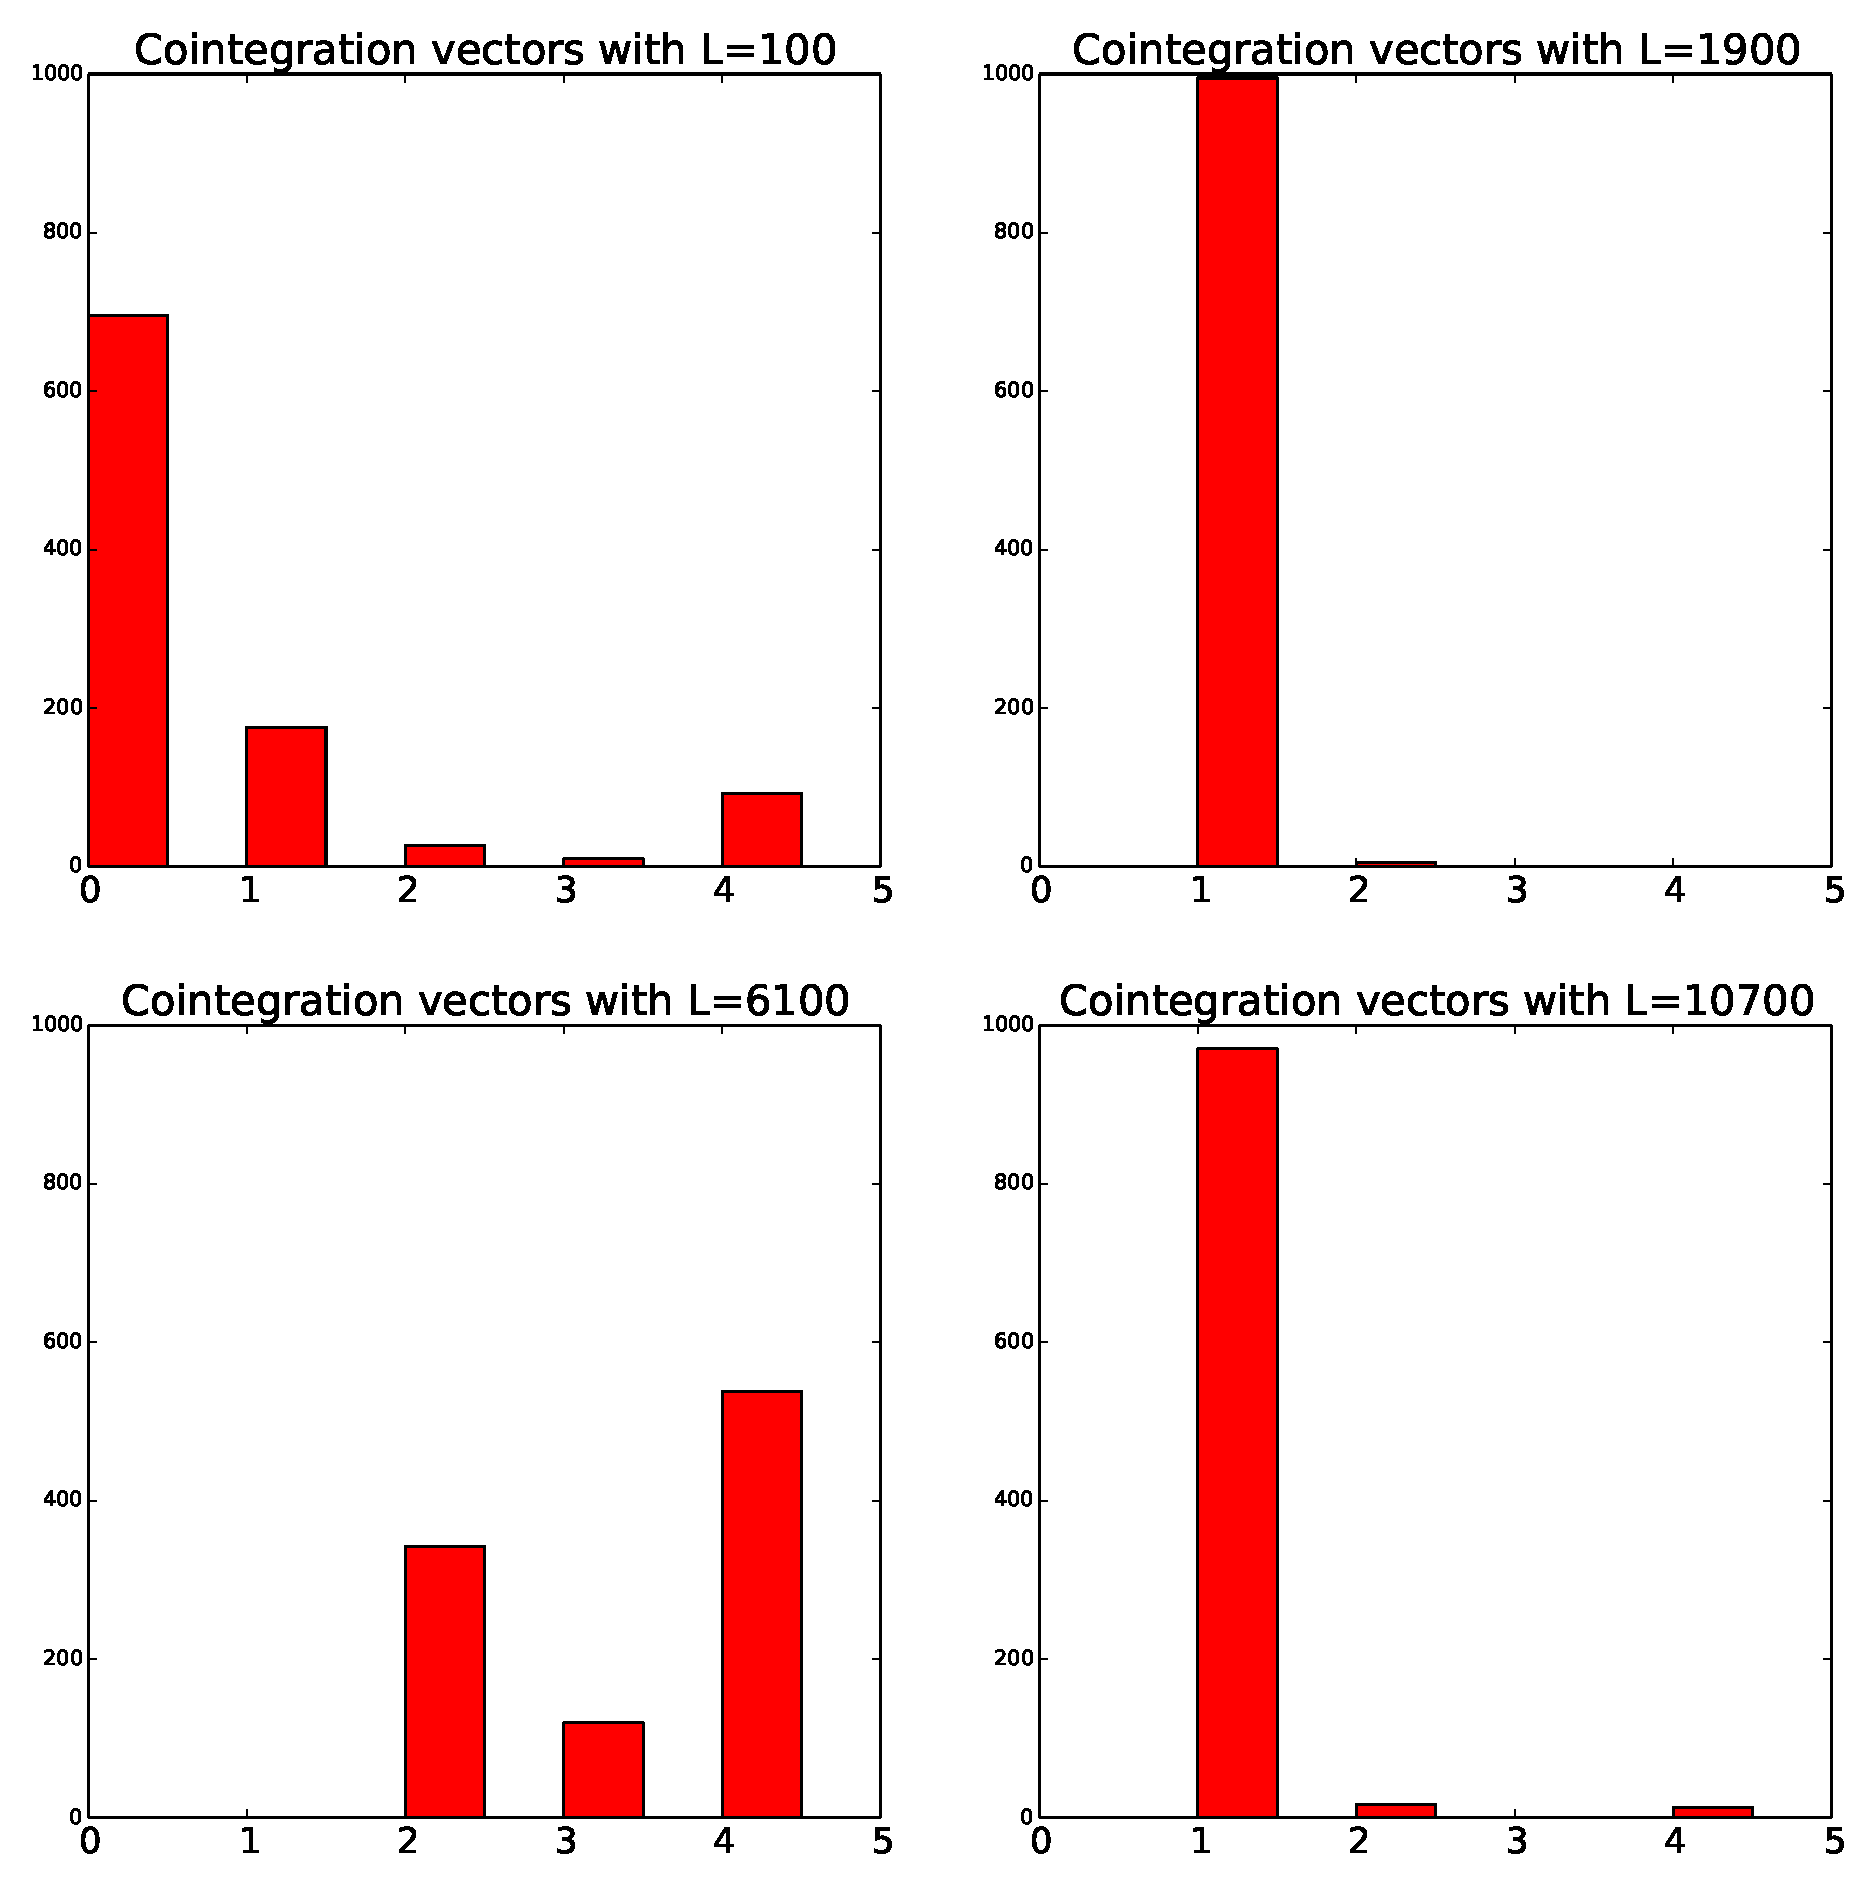
\includegraphics[width=\textwidth]{img/histCointVectors}
  \caption{Histogram of the number of cointegration vectors using $p=1$. Four
  possible values for $L$ are shown (100, 1900, 6100 and 10700).
  In the cases of $L=100$ and $L=6100$, most of the time there is little
  cointegration (0 or 4 cointegration vectors). However, for $L=1900$ and
  $L=10700$ significant cointegration is found.}
  \label{fig:hists}
\end{figure}

\begin{figure}[!h]
  %\vspace{-0.8cm}
  \centering
  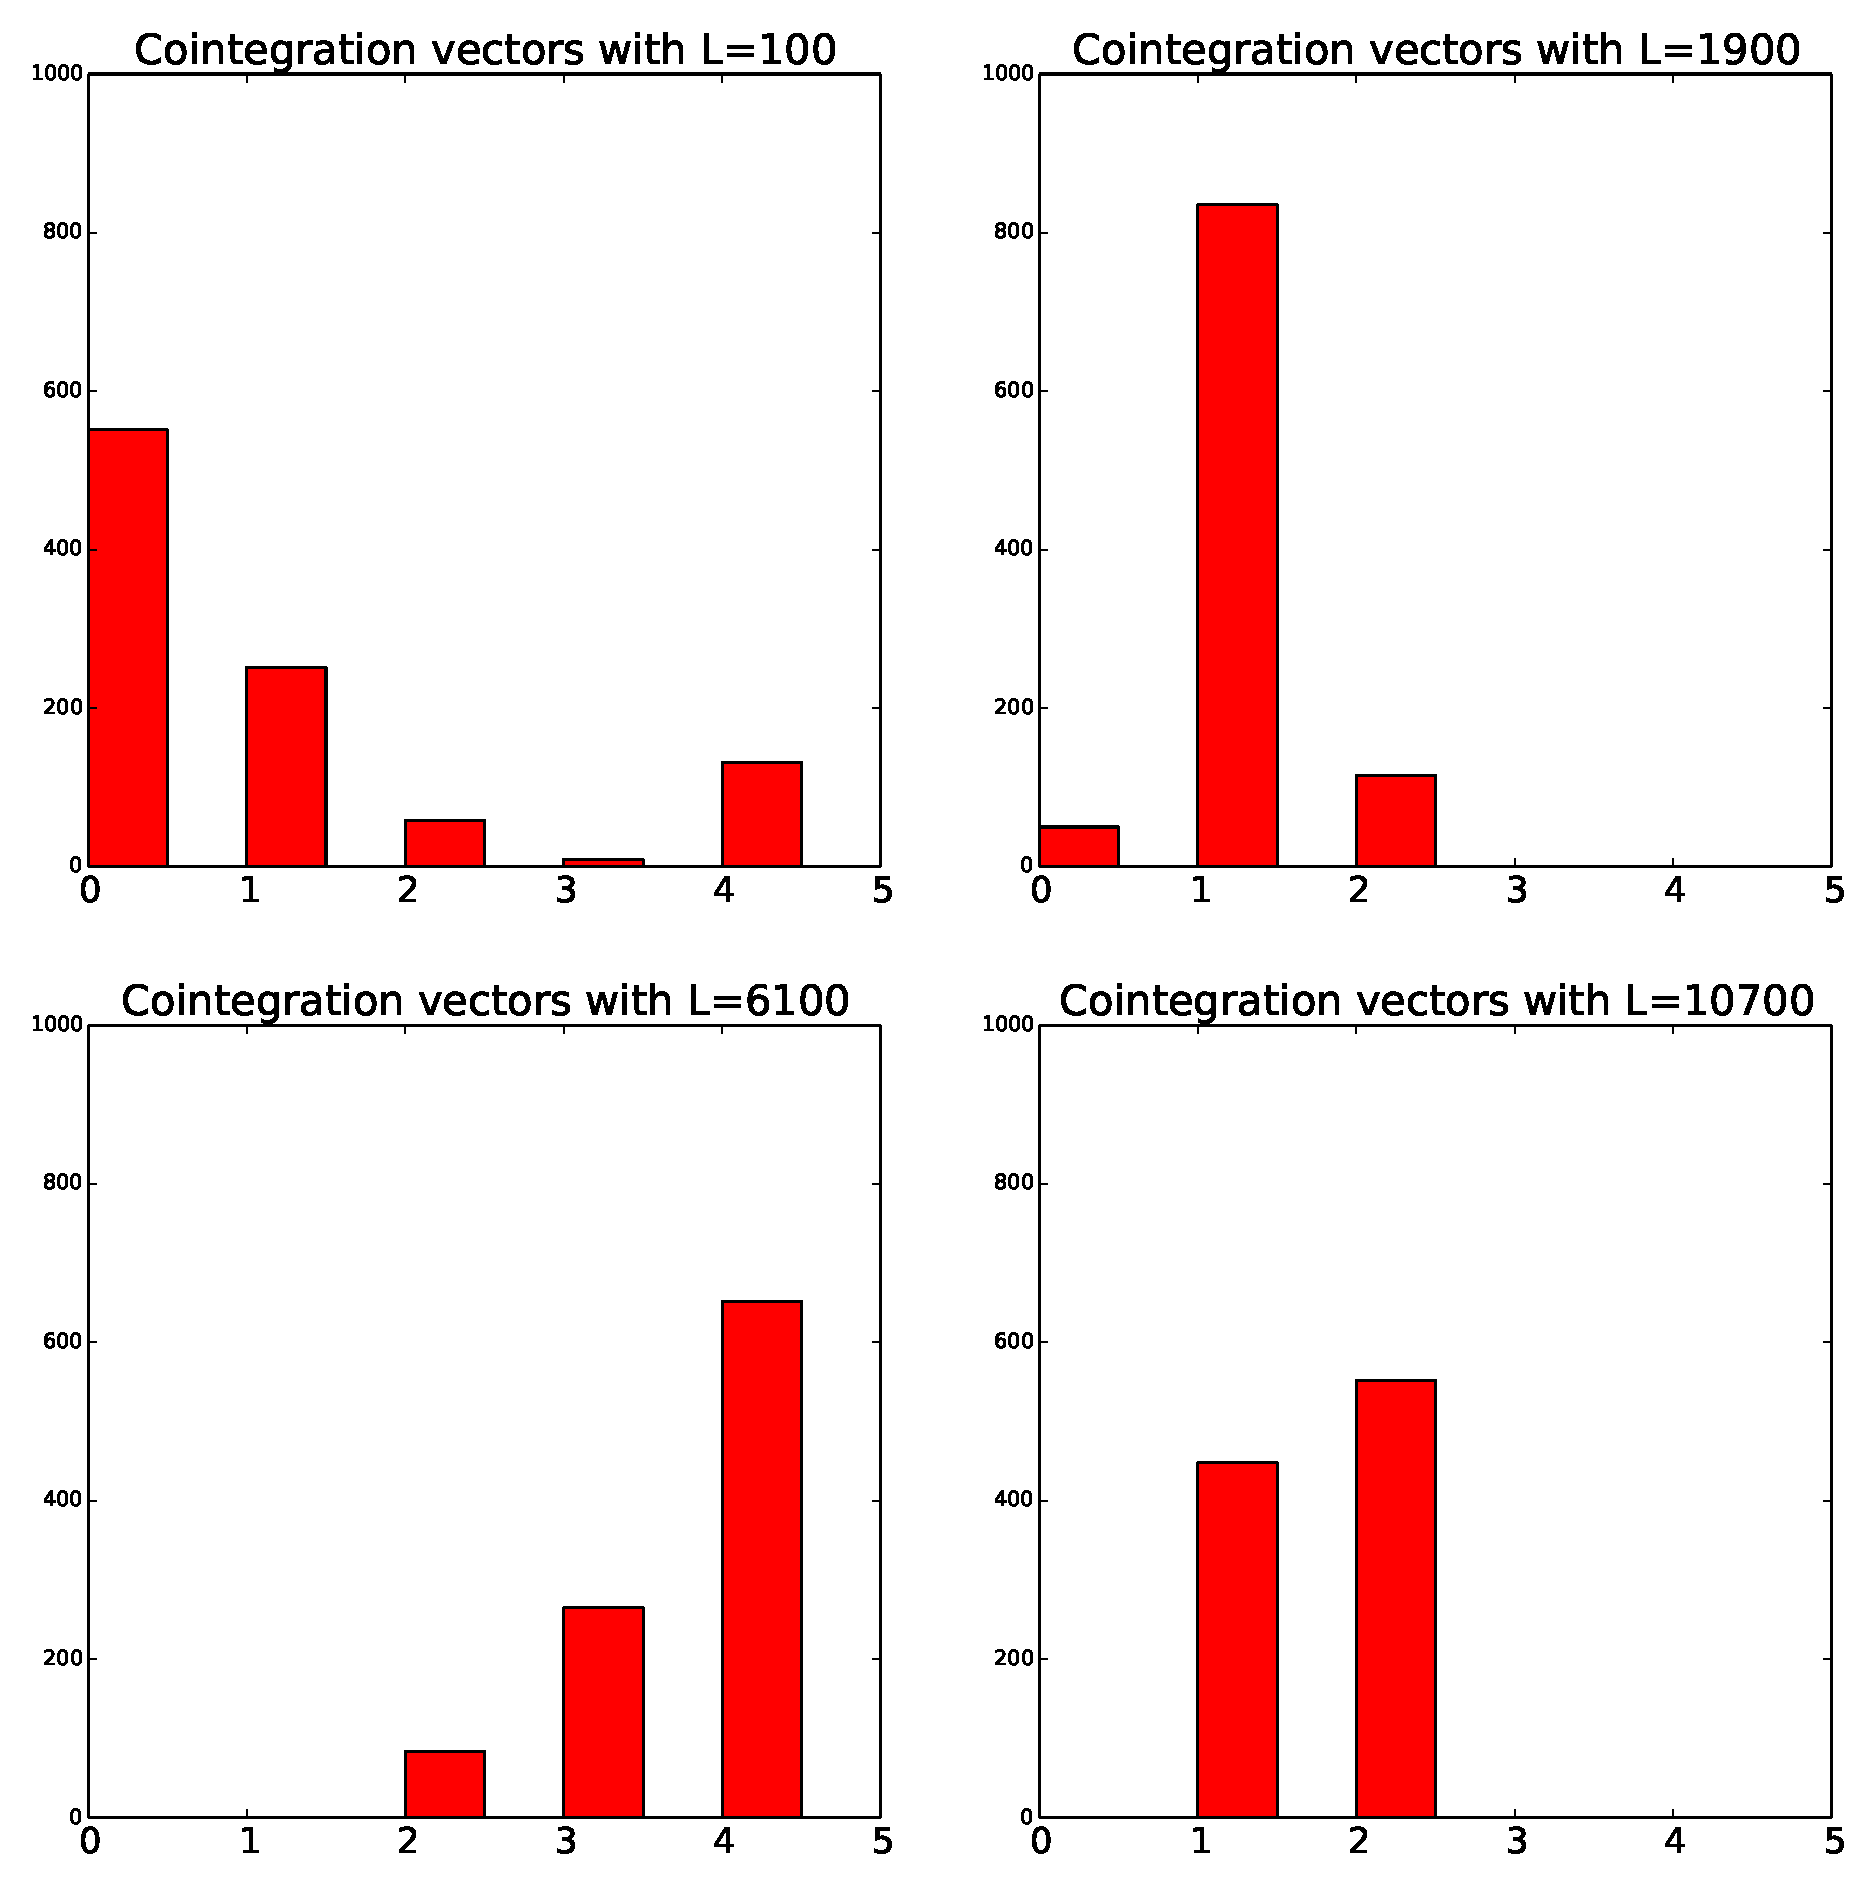
\includegraphics[width=\textwidth]{img/histCointVectorsp5}
  \caption{Histogram of the number of cointegration vectors using $p=5$. 
   Despite the change in the distribution of cointegration vectors, 
   the percentage of cointegration is nearly the same as in the case $p=1$. 
   For example, for $L=10700$ the sum of 1 and 2 number of cointegration
   vectors is very similar to 1 cointegration vector for the case $L=10700$
   in figure \ref{fig:hists}.}
   \label{fig:histsp5}
\end{figure}

The same experiments, using now $p=5$, were carried out in order to see the
effect on the number of cointegration vectors found. 
Figure~\ref{fig:histsp5} shows that, despite the change in the distribution
of the number of cointegration vectors, the sum of their number with $0<r<4$,
remain nearly the same. 
Therefore we can say that the number of lags doesn't significantly affect
the extent of cointegration found.

In order to measure the extent of cointegration, we introduce a
{\em percentage of cointegration\/} as following:
\begin{equation} \label{eq:pcoint}
PC = 
\frac{\#\{ it \mid \text{$it$ has $r$ c.v. with $0<r<l$}\}}
     {\#it}\times 100
\end{equation}
where c.v. stands for cointegration vectors and $it$ is the number of iterations.

The goal of our next experiment was to find a relation between this ratio
$PC$ and the performance of the accuracy measure MAPE (see equation 
\ref{eq:MAPE}). 
The experiments suggest that there is indeed a relation between the $PC$ ratio
and MAPE.
Figure~\ref{fig:cointvsmape} shows that MAPE rapidly decreases with increasing
$PC$.

\begin{figure}[!h]
  %\vspace{-0.8cm}
  \centering
  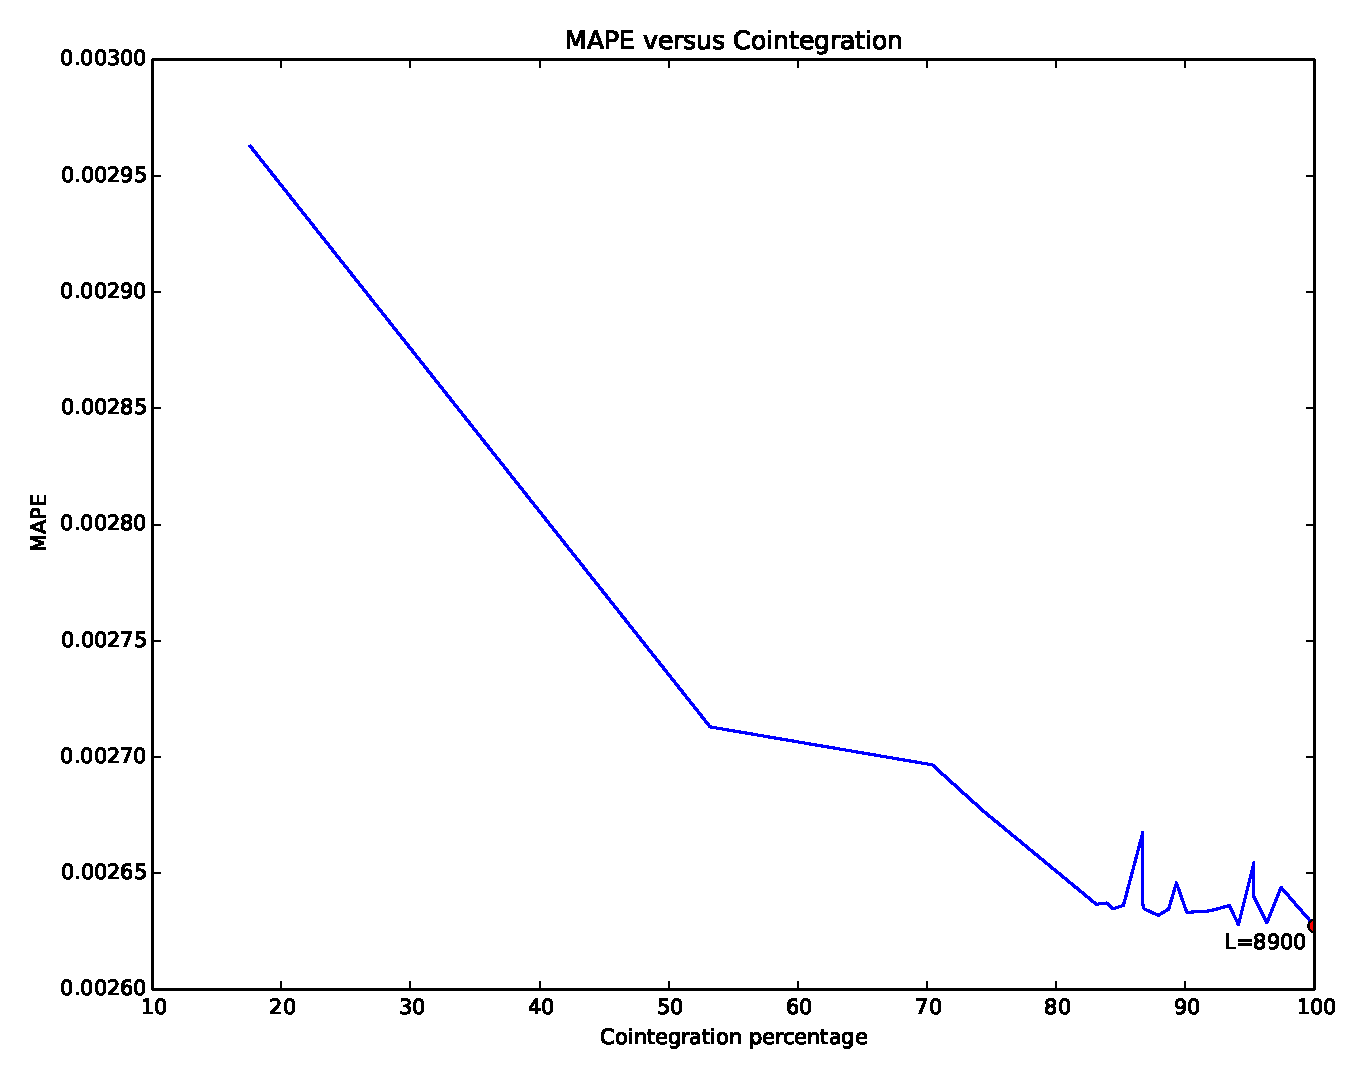
\includegraphics[width=0.8\textwidth]{img/MAPEvsCoint-offset21600-p-2-freq-10s}
  \caption{MAPE versus percentage of cointegration. MAPE was obtained from 1000
  iterations considering several possible $L=[100,10000,400]$ and $p=[1,5]$.
  Best $L$ found was 8900.}
  \label{fig:cointvsmape}
\end{figure}

From these results we observe that cointegration changes with different values
for $L$ and $p$ and also that better cointegration percentage leads to better
accuracy performance.
Therefore we propose to choose best $L$ and $p$ parameters determined at every
step. 
The criterion for choosing $L$ and $p$ is to maximise the percentage of
cointegration $PC$ considering a number of past iterations $it$.

Algorithm ~\ref{alg:AVECM} summarises our proposal. 
The function {\bf get\_best\_params} makes a grid search on the two vector
lists $Ls$ and $ps$ and returns the parameters $L$ and $p$ which maximise
the percentage of cointegration $PC$ (see equation~\ref{eq:pcoint}) for a
pre-defined number of iterations.
Since this search is computational expensive, the number of cointegration
vectors at each iteration is computed in parallel, thus ensuring a response
before new data is available. 
This parallel routine also allows to refine our grid search leading to obtain
improved forecasting performance.
After that optimum $L$ and $p$ parameters are found, VECM is built and used
to forecast next data.

\begin{algorithm}[ht]
\begin{algorithmic}[1]
\REQUIRE $\,$ \\
$\mathbf{y}$: matrix with $N$ input vectors and $l$ time series\\
$ps$: vector with the number of past values range \\
$Ls$: vector with window sizes range ($L<N$) \\
$outit$: Number of out-of-sample iterations($outit < N-L$)
$it$: Number of iterations of testing (in-sample)\\
$of$: Starting point of Testing \\
\ENSURE  $\,$ \\
$\{ \mathbf{y}_{\text{pred}}[1],\dots,\mathbf{y}_{\text{pred}}[N-L]\}$: model predictions 
\FOR { $i =of$ to $of + outit$ }
   \STATE $\mathbf{Y} \gets \mathbf{y}[i-\texttt{max}(Ls):i]$
    \STATE $L,p \gets
    \texttt{get\_best\_params}(Ls,ps,it,Y)$
    \STATE $\mathbf{y}_i \gets \mathbf{y}[i-L:i]$
        \STATE $model = VECM(\mathbf{y}_i, p)$
        \STATE $\mathbf{y}_{\text{pred}}[i] = model.predict()$
\ENDFOR
\end{algorithmic}
\caption{AVECM: Adaptive VECM.}
\label{alg:AVECM}
\end{algorithm}

%
%
%\subsection{Evaluation methods} \label{sec:evaluation}
%
%Forecast performance was evaluated using different methods. We chose three
%measures that are frequently used:
%\begin{description}
%\item
%{\bf MAPE}, Mean Average Percent Error, which presents forecast errors as a
%percentage:
%\begin{equation}\label{eq:MAPE}
%\text{MAPE} = \frac{1}{N} \sum_{t=1}^{N} 
%\frac{\left|\mathbf{y}_t-\hat{\mathbf{y}}_t\right|}{\left|\mathbf{y}_t\right|}
% \times 100 
%\end{equation}
%\item
%{\bf MAE}, Mean Average Error, which measures the distance between forecasts and the
%true value.
%\begin{equation}\label{eq:MAE}
%\text{MAE} = \frac{1}{N} \sum_{t=1}^{N} 
%\left| 
%\mathbf{y}_t-\hat{\mathbf{y}}_t
%\right| 
%\end{equation}
%\item
%{\bf RMSE}, Root Mean Square Error, also measures the distance between forecasts
%and the true values but, unlike MAE, large deviations from the true value have a
%large impact on RMSE due to squaring forecast error.
%\begin{equation}\label{eq:RMSE}
%\text{RMSE} = \sqrt{
%\frac{\displaystyle \sum_{t=1}^{N} (\mathbf{y}_t-\hat{\mathbf{y}}_t)^2}{N}}
%\end{equation}
%\end{description}
%
%
%
\section{Experimental results}
\label{sec:results}
\subsection{Data} \label{sec:unitroot}
AVECM tests were carried out using four foreign exchange rates all related to
USD: EURUSD, GBPUSD, USDCHF and USDJPY. This data was collected from the free
database Dukascopy which gives access to the Swiss Foreign Exchange marketplace
~\cite{Dukascopy2014}.

The tests were done using 10-seconds frequency from ask prices which
corresponded to 8640 data points per day from the 11th to the 15th of August
2014. Since data datetimes were in GMT, opening market times for London, New
York, Sidney and Tokyo corresponded with data points 1440, 3240, 6120 and 6840
respectively. Our tests were made considering two hours after the opening time
of the 13th of August. Therefore, in order to obtain these times, we added 2
days and 2 hours to all the opening times ($2\times 8640 + 2 \times 360$) to obtain:
19440, 21240, 24120 and 24840. We called offset to these times in
table~\ref{tab:stats}, which allowed us to obtain performance at different
times of the day.

\subsection{Unit root tests} \label{sec:unitroot}
Before running the tests, we firstly checked whether the time series were
I(1) using the Augmented Dickey Fuller (ADF) test at 95\% significance level.
Table~\ref{tab:adf} shows that all currency rates cannot reject the unit root
test but they rejected it with their first differences. This means that all of
them are I(1) time series and we are allowed to use VECM and therefore AVECM.

\begin{table}[h!]
\begin{center}
\begin{tabular}{|l|c|c|c|c|c|}
\hline
& \textbf{Statistic} & \textbf{Critical value} & \textbf{Result}\\
\hline
EURUSD          &  -0.05398   & -1.94101 & True       \\
$\Delta$ EURUSD & -89.12344   & -1.94101 & False       \\
GBPUSD          &  -0.88208   & -1.94101 & True          \\
$\Delta$ GBPUSD & -82.56501   & -1.94101 & False       \\
CHFUSD          & -0.49941    & -1.94101 & True         \\
$\Delta$ CHFUSD & -74.21940   & -1.94101 & False       \\
JPYUSD          &  0.36721    & -1.94101 & True        \\
$\Delta$ JPYUSD & -101.15589  & -1.94101 & False     \\ 
\hline
\end{tabular}
\end{center}
\caption{Unit roots tests for EURUSD, GBPUSD, USDCHF and USDJPY at 10-seconds
frequency.}
\label{tab:adf}
\end{table}


\section{Parallel implementation} \label{sec:paralell}

To determine optimal $L$ and $p$ parameters require the using of the Johansen
method which is a computationally expensive routine. 
In order to improve the execution time of this search, our proposal included
a parallel search of VECM parameters using high performance computing.
The main objective is to obtain a response before a new data arrives in
the next 10 seconds.

The Johansen method is implemented in the Python Statsmodels
library~\cite{seabold2010} and the parallel implementation was done using
MPI in Python. 
MPI was chosen because it allows large-scale parallel applications
with wide portability to be built, being able to run in large clusters
or on local computers.
Our tests were done in a cluster with 2 servers Xeon E5-2667 (2.90GHz)
of 24 cores each (48 cores in total) and 24GB RAM.

Since financial market are constantly changing, we ran our
algorithm using different times of the day. We chose to use the algorithm
starting on the third day and two hours after the market opening times. These
times corresponded to data points 19440 (5 GMT London), 21240 (10 GMT New
York), 24120 (19 GMT Sydney) and 24840 (9 GMT Tokyo).

In order to determine the percentage of cointegration vectors, we considered
different number of iterations: 10, 50 and 100. The number of possible
combinations ($nparam$) of $L$ and $p$ is shown for 12, 24 and 47.


\subsection{Performance accuracy} \label{sec:performacc}

Table~\ref{tab:stats} shows the out-of-sample performance measures: MAPE, MAE
and RMSE for AVECM for different offsets, iterations and number of parameters.
We observed that performance measures differ for different offsets having even
in some cases different orders. London and New York offsets are order $10^{-3}$
while Sidney and Tokyo vary between $10^{-3}$ and $10^{-4}$. Despite this
difference in the order, they all achieve their minimum MAPE, MAE and RMSE
measurements at 100 iterations. In the case of Tokyo, it also reduces its MAPE
order. In all cases, we can see that performance measures are improving with
the number of parameters.  This is because there are more possible options to find
optimal cointegration parameters.

Figure ~\ref{fig:accuracy} shows part of the out-of-sample forecasts made by
our proposed AVECM using 100 iterations and offset New York.

\begin{figure}[!h]
  \centering
  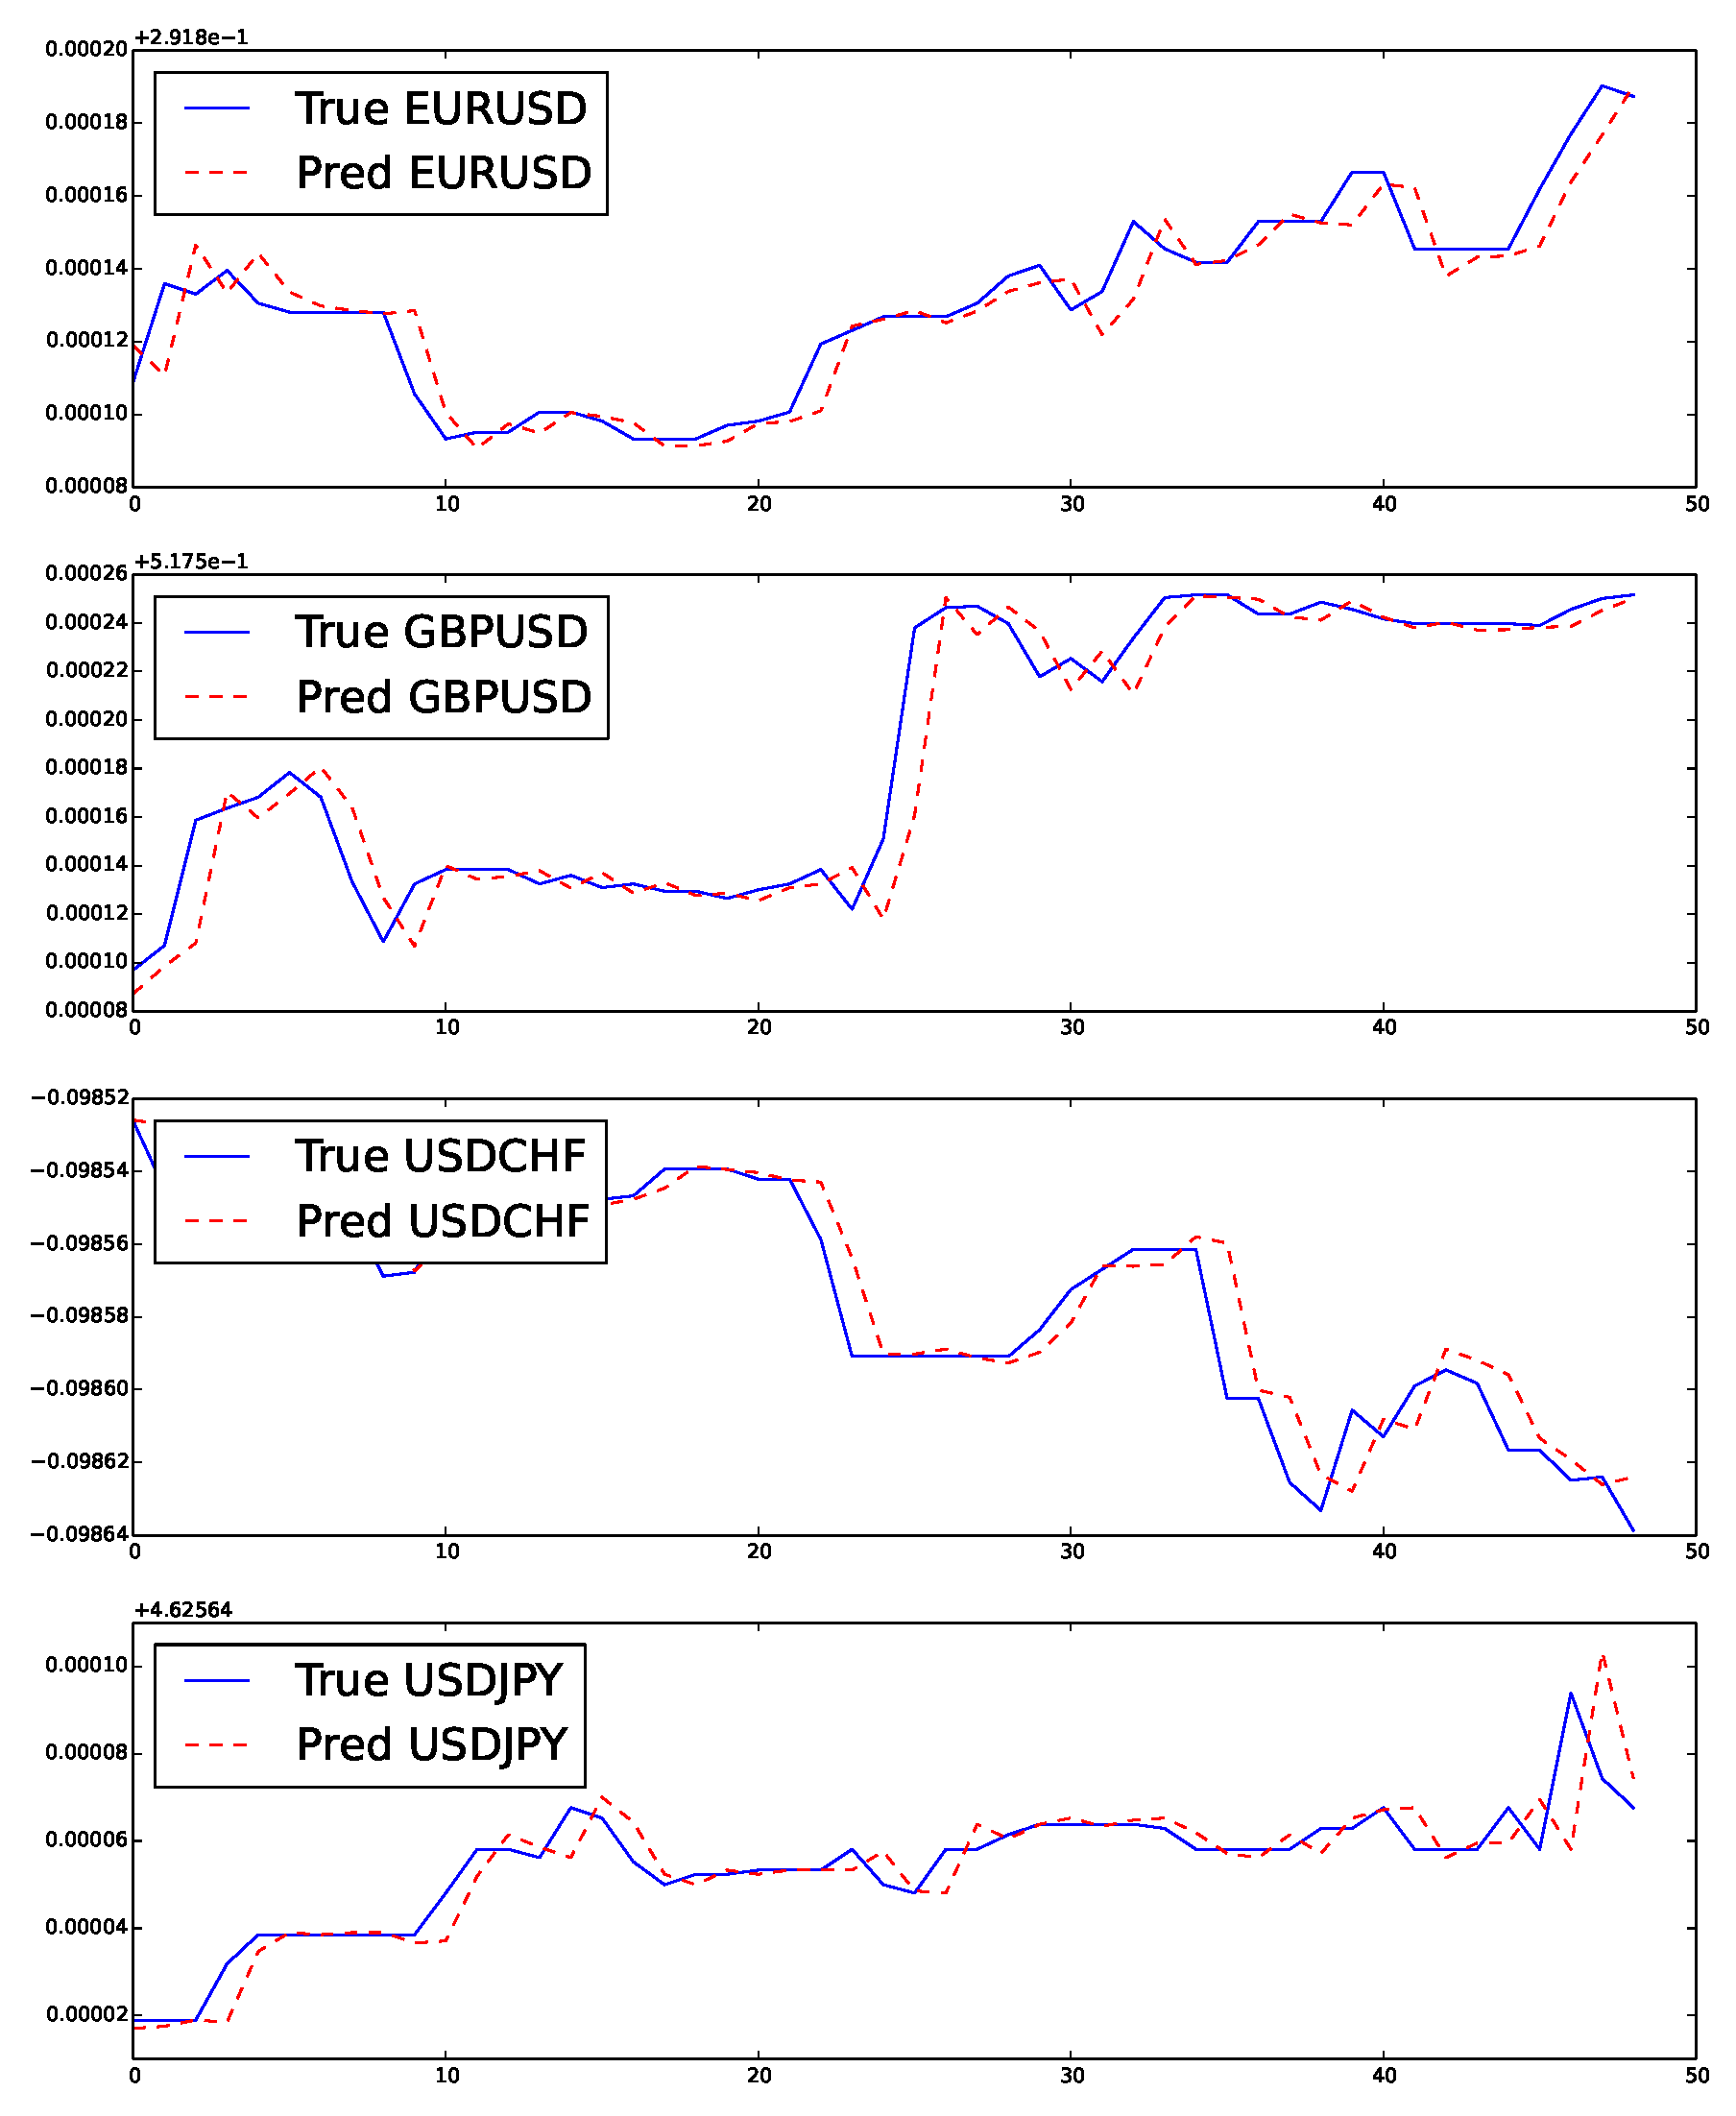
\includegraphics[width=\textwidth]{img/accuracy}
  \caption{AVECM out-of-sample forecasting for four currency rates.}
  \label{fig:accuracy}
\end{figure}


\begin{table*}[ht!]
\tiny
\caption{Performance and execution times for min MAPE criteria}
\label{tab:stats}
\begin{center}
\begin{tabular}{|l|l|l|c|c|c|c|c|}
\hline
\multicolumn{3}{|c}{Parameters} & 
\multicolumn{3}{|c}{Out-of-sample Performance} &
\multicolumn{2}{|c|}{Time[s]} \\ 
\hline

\hline
Offset & Iterations & $nparam$ & 
MAPE & MAE& RMSE& 
Sequencial & Parallel \\
\hline
 \multirow{12}{*}{19440 (London)} &
 \multirow{3}{*}{10} 
  &  12 & 1.8481E-03 & 5.1974E-04 & 7.9714E-04 & 2.64 & 2.61    \\
 &&  24 & 1.8793E-03 & 5.2935E-04 & 8.0128E-04 & 7.38 & 3.03 \\ 
 &&  47 & 1.8804E-03 & 5.2477E-04 & 7.9274E-04 & 18.86 & 3.07 \\ 
 \cline{2-8} 
 & \multirow{3}{*}{50} 
 &  12&  1.5760E-03 & 3.8559E-04 & 6.5579E-04 & 12.49 & 3.99 \\
 && 24 & 1.5645E-03 & 3.7379E-04 & 6.3128E-04 & 36.69 & 6.45 \\
 && 47 & 1.5757E-03 & 3.7336E-04 & \textbf{6.2828E-04} & 92.30 & 5.75 \\
 \cline{2-8} 
 & \multirow{3}{*}{100} 
 &  12&  1.5760E-03 & 3.8559E-04 & 6.5579E-04 & 25.00 & 5.90 \\ 
 && 24 & \textbf{1.5501E-03} & \textbf{3.6575E-04} & 6.4058E-04 & 70.58 & 9.74 \\ 
 && 47 & 1.5812E-03 & 3.8773E-04 & 6.4740E-04 & 185.05 & 11.09 \\
 \cline{2-8} 
 & \multirow{3}{*}{150} 
 &  12&  1.5760E-03 & 3.8559E-04 & 6.5579E-04 & 37.09 & 7.55 \\ 
 && 24 & 1.5501E-03 & 3.6575E-04 & 6.4058E-04 & 104.52 & 14.33 \\
 && 47 & 1.5812E-03 & 3.8773E-04 & 6.4740E-04 & 292.84 & 15.44 \\
\hline
\hline
 \multirow{12}{*}{21240 (New York)} &
 \multirow{3}{*}{10} 
  &  12 & 1.8358E-03 & 3.4906E-04 & 4.9314E-04 & 2.64 & 2.45 \\
 &&  24 & 1.8287E-03 & 3.4661E-04 & 4.9140E-04 & 7.38 & 3.03 \\
 &&  47 & 1.8402E-03 & 3.4937E-04 & 4.9298E-04 & 18.86 & 3.00 \\
 \cline{2-8} 
 & \multirow{3}{*}{50} 
 &  12&  1.6911E-03 & 3.3614E-04 & 4.8197E-04 & 12.49 & 4.00 \\
 && 24 & 1.6871E-03 & 3.3546E-04 & 4.8198E-04 & 36.69 & 6.15 \\
 && 47 & 1.6991E-03 & 3.3790E-04 & \textbf{4.8141E-04} & 92.30 & 6.17 \\
 \cline{2-8} 
 & \multirow{3}{*}{100} 
 &  12&  1.6911E-03 & 3.3614E-04 & 4.8197E-04 & 25.00 & 6.03 \\ 
 && 24 & \textbf{1.6857E-03} & \textbf{3.3510E-04} & 4.8308E-04 & 70.58 & 9.34 \\ 
 && 47 & 1.6978E-03 & 3.3766E-04 & 4.8285E-04 & 185.05 & 10.36 \\
 \cline{2-8} 
 & \multirow{3}{*}{150} 
 &  12& 1.6911E-03 & 3.3614E-04 & 4.8197E-04 & 37.09 & 7.77 \\   
 && 24 &1.6857E-03 & 3.3510E-04 & 4.8308E-04 & 104.52 & 13.84 \\
 && 47 &1.6978E-03 & 3.3766E-04 & 4.8285E-04 & 292.84 & 13.06 \\
\hline
\hline
 \multirow{12}{*}{24120 (Sidney)} &
 \multirow{3}{*}{10} 
  &  12 & 8.5847E-04 & 2.2284E-04 & 3.1202E-04 & 2.64 & 2.41 \\ 
 &&  24 & 7.9127E-04 & 1.9526E-04 & 2.9580E-04 & 7.38 & 2.86 \\ 
 &&  47 & 8.0491E-04 & 1.9578E-04 & 2.9669E-04 & 18.86 & 3.13 \\ 
 \cline{2-8} 
 & \multirow{3}{*}{50} 
 &  12& 9.1471E-04 & 2.2555E-04 & 3.1371E-04 & 12.49 & 4.02 \\ 
 && 24 &7.3172E-04 & 1.8017E-04 & 2.8054E-04 & 36.69 & 5.45 \\
 && 47 &7.3172E-04 & 1.8017E-04 & 2.8054E-04 & 92.30 & 6.48 \\
 \cline{2-8} 
 & \multirow{3}{*}{100} 
 &  12& 8.0458E-04 & 2.0706E-04 & 2.9542E-04 & 25.00 & 5.90 \\ 
 && 24 &\textbf{6.2547E-04} & 1.6451E-04 & 2.5945E-04 & 70.58 & 9.23 \\ 
 && 47 &6.3424E-04 & \textbf{1.6400E-04} & \textbf{2.5849E-04} & 185.05 & 11.13 \\
 \cline{2-8} 
 & \multirow{3}{*}{150} 
 &  12&  7.2437E-04 & 1.8782E-04 & 2.8016E-04 & 37.09 & 7.83 \\ 
 && 24 & 6.2547E-04 & 1.6451E-04 & 2.5945E-04 & 104.52 & 12.42 \\
 && 47 & 6.2547E-04 & 1.6451E-04 & 2.5945E-04 & 292.84 & 13.95 \\
\hline
\hline
 \multirow{12}{*}{24840 (Tokyo)} &
 \multirow{3}{*}{10} 
  &  12 & 1.0787E-03 & 3.3948E-04 & 5.5145E-04 & 2.64 & 2.45 \\ 
 &&  24 & 1.0823E-03 & 3.3992E-04 & 5.4697E-04 & 7.38 & 2.96 \\ 
 &&  47 & 1.0885E-03 & 3.4462E-04 & 5.5231E-04 & 18.86 & 3.05 \\
 \cline{2-8} 
 & \multirow{3}{*}{50} 
 &  12& 1.0753E-03 & 3.4955E-04 & 5.7100E-04 & 12.49 & 3.97 \\ 
 && 24 &1.1042E-03 & 3.5395E-04 & 5.6747E-04 & 36.69 & 6.08 \\ 
 && 47 &1.1238E-03 & 3.5794E-04 & 5.7330E-04 & 92.30 & 6.67 \\ 
 \cline{2-8} 
 & \multirow{3}{*}{100} 
 &  12& \textbf{8.4691E-04} & \textbf{2.8979E-04} & \textbf{5.2553E-04} & 25.00 & 5.74 \\ 
 && 24 &8.6649E-04 & 2.9405E-04 & 5.2874E-04 & 70.58 & 10.29 \\
 && 47 &8.8877E-04 & 2.9821E-04 & 5.3796E-04 & 185.05 & 9.00 \\
 \cline{2-8} 
 & \multirow{3}{*}{150} 
 &  12& 8.5021E-04 & 2.9579E-04 & 5.2707E-04 & 37.09 & 7.54 \\ 
 && 24 &8.6350E-04 & 2.9183E-04 & 5.2837E-04 & 104.52 & 13.05 \\
 && 47 &8.8597E-04 & 2.9594E-04 & 5.3759E-04 & 292.84 & 13.82 \\
\hline
\end{tabular}
\end{center}
\end{table*}





\subsection{Execution times} \label{sec:exectimes}
We ran AVECM 100 ($outit$ in algorithm~\ref{alg:AVECM}) iterations.
Table~\ref{tab:stats} shows execution times and performance measures for
different times of the market, in-sample iterations and number of parameters used.
The number of parameters represents the possible combinations of values for $L$ and
$P$. The $L$ parameter was always chosen between 100 and 4000 and $nparams$
determines how many values in this range were considered. $p$ always took values
between 1 and 5. Execution times were measured using the Time python library.

Execution time depends directly on $L$ and $p$ since they determine the size of
matrix $\mathbf{A}$ and therefore affects the OLS function execution time.
Therefore, if we try more combinations of $L$ and $p$ (increasing $nparam$) the
algorithm will take longer. However, the idea is to improve accuracy measures
ensuring execution times below 10 seconds (the time series frequency). 

Table ~\ref{tab:stats} shows that best performance accuracy measures are
achieved in times near or below 10 seconds in the parallel version. Contrarily,
sequential times are high, above 10 seconds in most of the cases.

Despite there being some parallel execution times above 10 seconds, the
performance measures didn't improve and so they can be dismissed.

Figure~\ref{fig:extimes} shows sequential and parallel time and speed-up
computing time for VECM with 100 iterations.

\begin{figure}[!h]
  \centering
  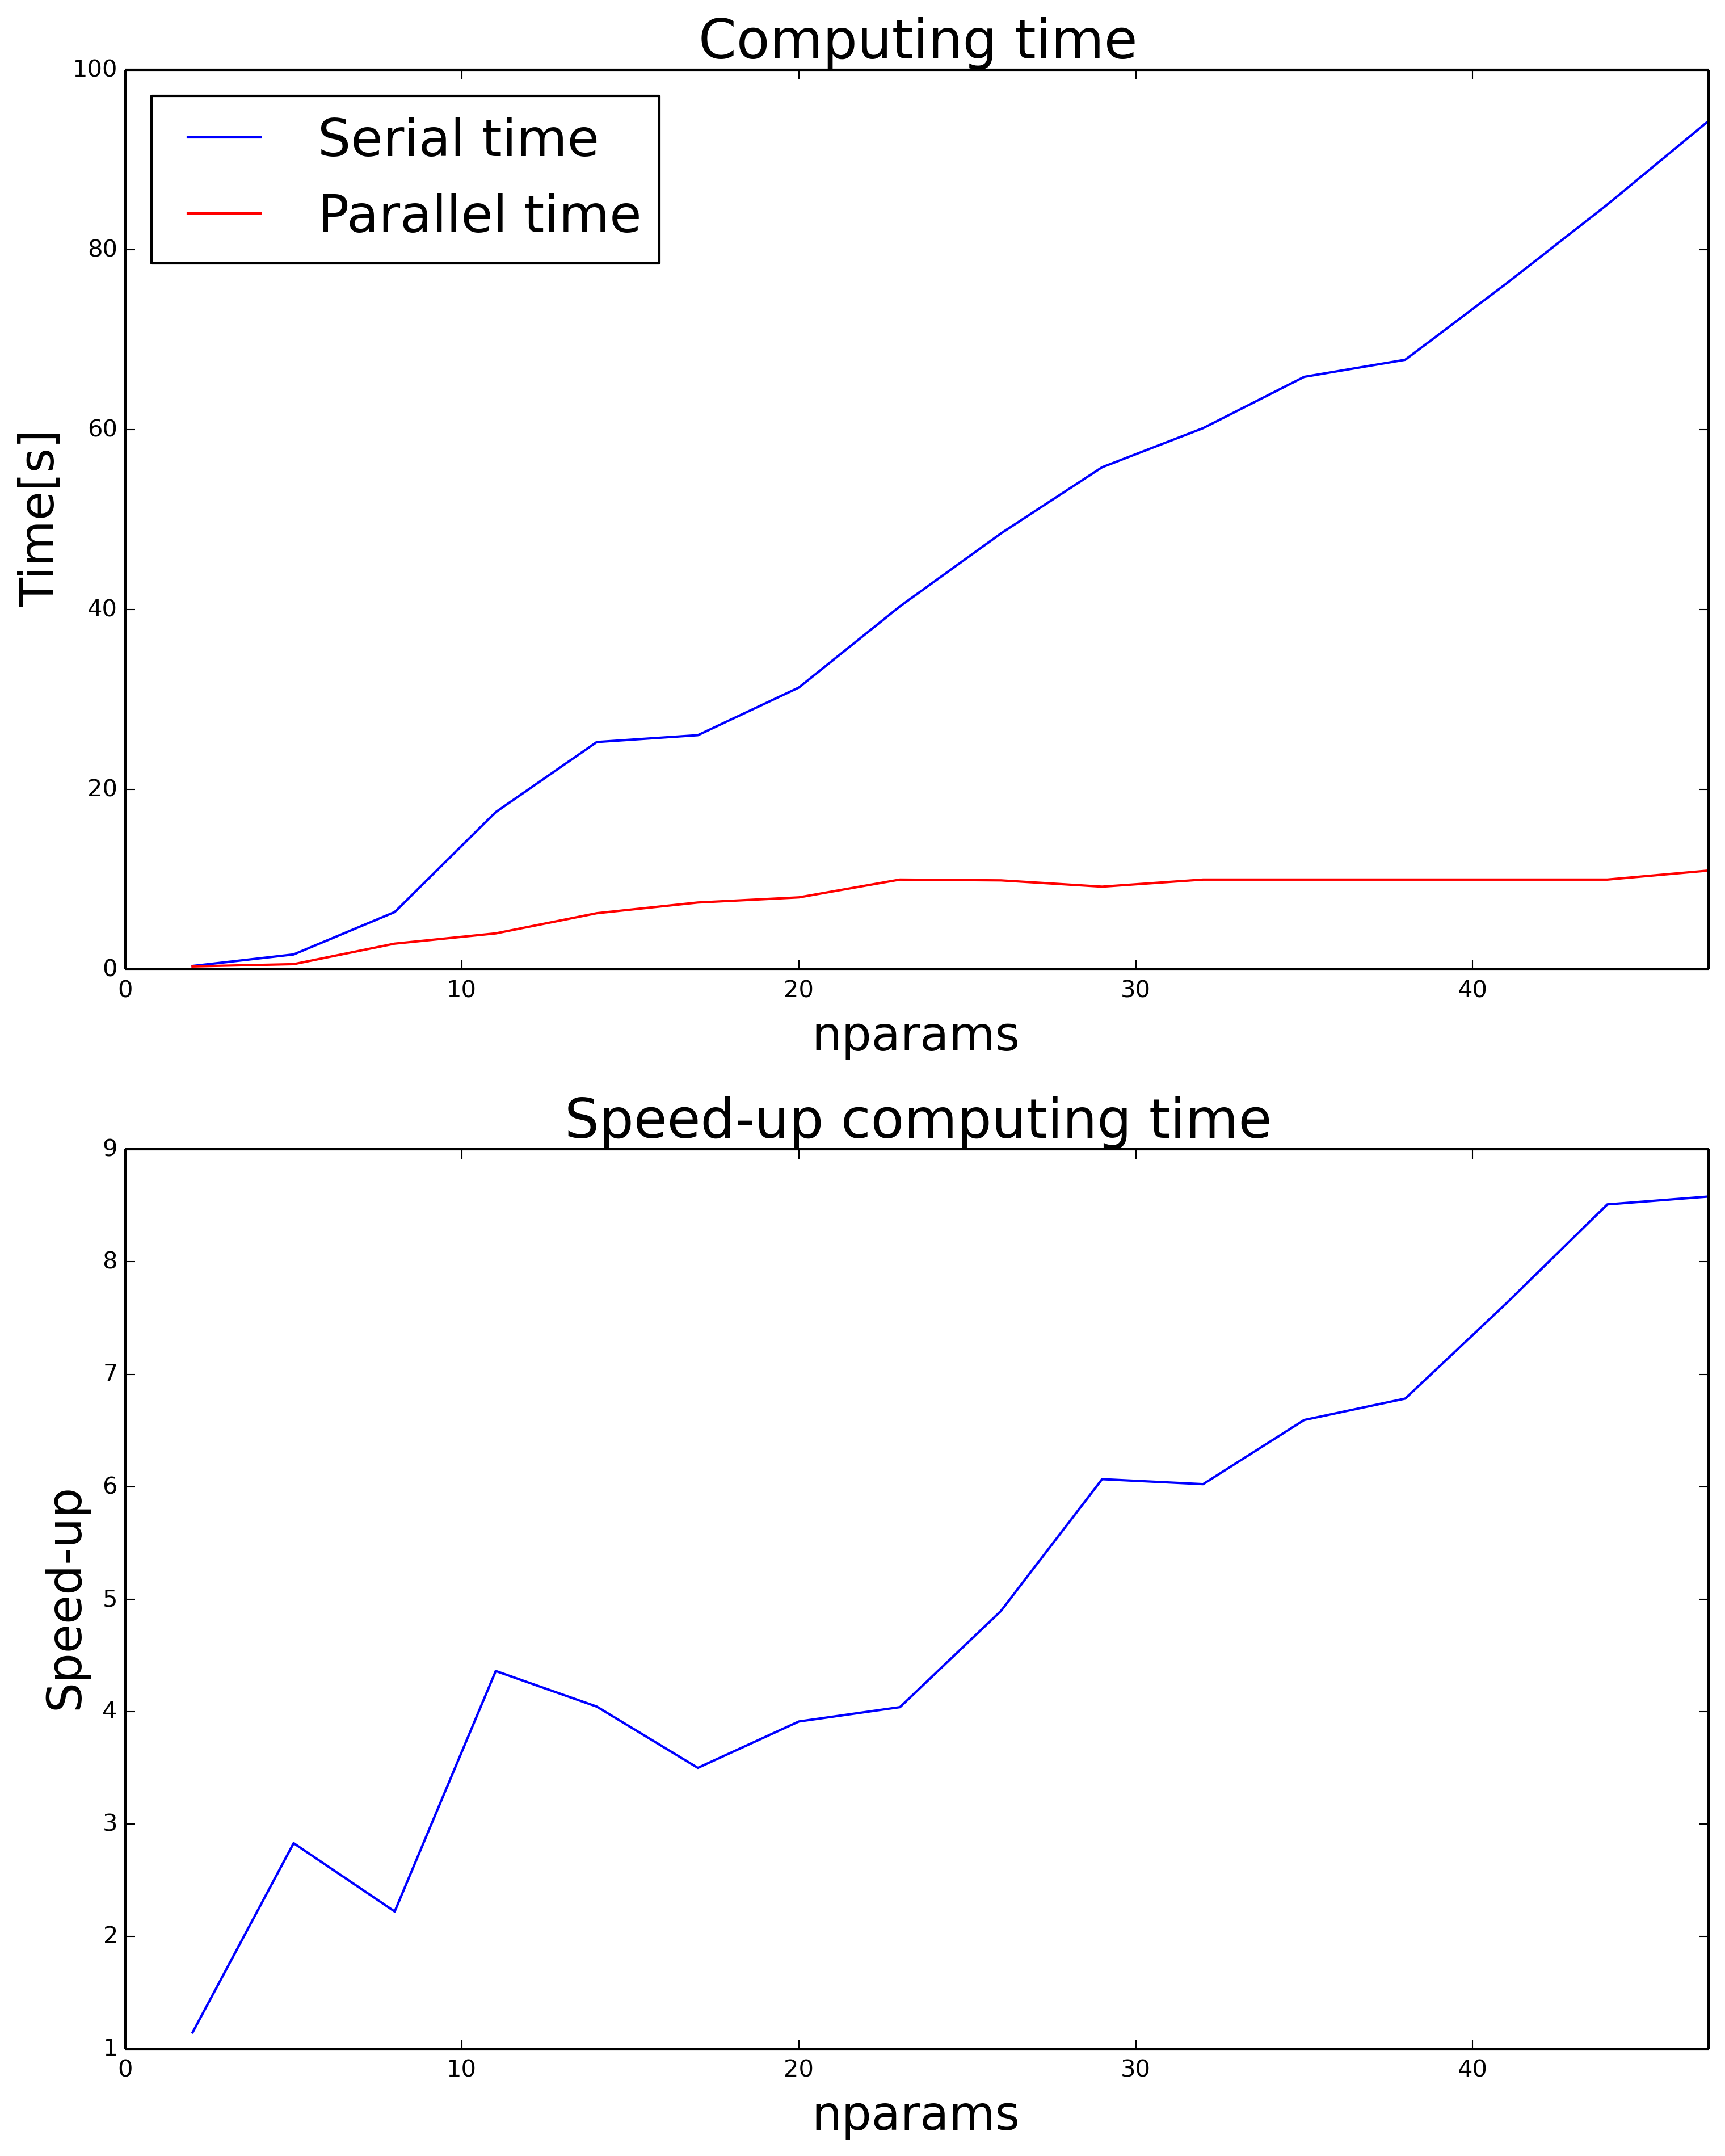
\includegraphics[width=0.7\textwidth]{img/extimes}
  \caption{Computing time of sequential and parallel algorithm is shown in the
  upper figure. Speed-up is shown below.}
  \label{fig:extimes}
\end{figure}


Execution times do not consider the loading data time, just the finding of
best parameters and the building the VECM model. The time MPI spends
transferring data and synchronising process is about two seconds independently
of the number of process considered.

\section{Conclusions}
\label{sec:conclusions}
Cointegration in financial time series has been largely studied and the 
Johansen method is commonly used to obtain it. 
In practice it has been found that cointegration relations change with time. 
However, cointegration model-based such as VECM assumes that cointegration
remains unchanged in time. 
We empirically showed that the Johansen method is sensitive to the number
of lags but also to the amount of data considered.

Moreover, we introduced the notion of {\em percentage of cointegration\/} and
have found that out-of-sample forecast performance is related to the value of
this figure in the last samples.  We used this information to set the model
parameters.  Our proposal AVECM consists then on an adaptive algorithm to update VECM
parameters every time that new data is available. These parameters are found by
maximising the percentage of cointegration of the last samples or iterations.

Determining VECM parameters was the most expensive routine and it was run
using parallel processes using MPI which allowed a grid search within a range of
values for $L$ and $p$ to be made.
Tests were done using real currency rates data. 
Our proposal was tested in several scenarios using different times of
the day to show its behaviour related to the opening times of
financial markets.

Results showed that our proposed AVECM improves performance measures by finding
parameters of $L$ and $p$ maximising the percentage of cointegration.
These facts were consistent for different times of the day. 
We found that increasing the number of parameters will always lead to
better performance measures. Furthermore, in the case of Tokyo 
financial market opening time, MAPE reduced an order from $10^{-3}$ to $10^{-4}$.

The parallel implementation allowed the execution times to be reduced
more than ten times and therefore a response time was obtain before 10
seconds. Since we used 10-second frequency we can say that our proposal is suitable
for use in an online context for real applications because response times
were less than this frequency.

For future study, it would be interesting to explore the relation between
cointegration and performance in order to propose new criteria for
improving VECM parameters.


